%!TEX program=xelatex

\documentclass[11pt]{ctexart}  
\usepackage[top=2cm, bottom=2cm, left=2cm, right=2cm]{geometry}  
\usepackage{algorithm}  
\usepackage{algorithmicx}  
\usepackage{algpseudocode}  
\usepackage{amsmath}  
\usepackage{graphicx}
\usepackage{amsmath}
\usepackage{amssymb}


\floatname{algorithm}{算法}
\renewcommand{\algorithmicrequire}{\textbf{输入:}}  
\renewcommand{\algorithmicensure}{\textbf{输出:}} 

\title{密码学实验报告4}
\author{张天辰 17377321}

\makeatletter
\newenvironment{breakablealgorithm}
  {% \begin{breakablealgorithm}
   \begin{center}
     \refstepcounter{algorithm}% New algorithm
     \hrule height.8pt depth0pt \kern2pt% \@fs@pre for \@fs@ruled
     \renewcommand{\caption}[2][\relax]{% Make a new \caption
       {\raggedright\textbf{\ALG@name~\thealgorithm} ##2\par}%
       \ifx\relax##1\relax % #1 is \relax
         \addcontentsline{loa}{algorithm}{\protect\numberline{\thealgorithm}##2}%
       \else % #1 is not \relax
         \addcontentsline{loa}{algorithm}{\protect\numberline{\thealgorithm}##1}%
       \fi
       \kern2pt\hrule\kern2pt
     }
  }{% \end{breakablealgorithm}
     \kern2pt\hrule\relax% \@fs@post for \@fs@ruled
   \end{center}
  }
\makeatother

\begin{document}
\maketitle{}



\section{DES算法}
\subsection{简介}
DES是针对64bit明文和64bit密钥的基于Feistel结构的分组加密方案。该算法先将密钥进行PC1变换后分成两半每次循环左移特定位数再进行PC2变换生成16个子密钥。然后将明文进行IP置换,每轮加密结果的左半部分就是上一轮的右半部分,右半部分是左部分与右部分经过f函数后异或的结果。最后再将得到的左右部分互换,并进行IP逆置换就得到密文。DES加密算法与解密算法相同,只是子密钥使用顺序完全相反。
\subsection{算法实现}
\begin{breakablealgorithm}  
    \caption{DES}  
    \begin{algorithmic}[1] %每行显示行号  
        \Require 明文$src\_message$(加密),密钥$src\_key$,密文$src\_cipher$(解密)  
        \Ensure 密文$cipher$(加密),明文$message$(解密)
        \Function {generate\_key}{$src\_key$} 
            \State $bin\_key \gets 64bit的src\_key$
            \State $key \gets 变换PC1(bin\_key)$
            \State $keys \gets key$左右两半进行特定次循环左移生成的56bit值
            \State $keys$每项进行PC2变换
            \State \Return $keys$
        \EndFunction
        \Function {f}{$right, key$}
            \State $b \gets key \oplus 变换E(right)$
            \State $c \gets b$分8部分进入S盒
            \State \Return 变换$P(c)$
        \EndFunction
        \Function {DES\_encrypt}{$src\_message, src\_key$}
            \State $keys \gets$\Call{generate\_key}{$src\_key$}
            \State $message \gets src\_message$转换为64bit二进制后再进行IP变换
            \State $left \gets message[0:32]$
            \State $right \gets message[32:]$
            \For {each $i \in [0, 16)$}
                \State $left, right \gets right, left \oplus $\Call{f}{right, keys[i]}
            \EndFor
            \State \Return 变换$IP^{-1}(right + left)$
        \EndFunction
        \Function {DES\_decrypt}{$src\_cipher, src\_key$}
            \State $keys \gets$\Call{generate\_key}{$src\_key$}逆序
            \State $cipher \gets src\_cipher$转换为64bit二进制后再进行IP变换
            \State $left \gets cipher[0:32]$
            \State $right \gets cipher[32:]$
            \For {each $i \in [0, 16)$}
                \State $left, right \gets right, left \oplus $\Call{f}{right, keys[i]}
            \EndFor
            \State \Return 变换$IP^{-1}(right + left)$
        \EndFunction
    \end{algorithmic}  
\end{breakablealgorithm}

\subsection{测试样例}
\begin{figure}[htbp]
\centering
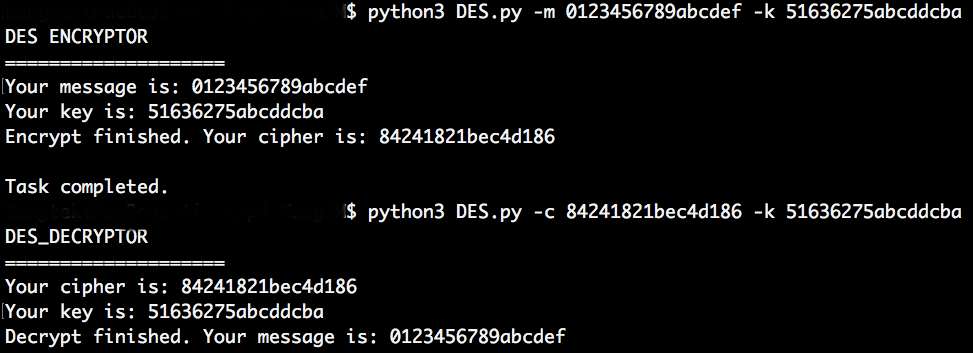
\includegraphics[height=3.53cm,width=9.73cm]{des.png}
\caption{DES}
\label{des}
\end{figure}



\section{DES差分攻击}
\subsection{简介}
DES差分攻击的基础是,对于同一个S盒,不同输入异或的输出异或分布并不均匀,因此可以大大减少穷举范围。对于三轮DES,最后一轮的输入异或可以从密文的左半部分经过E变换得到,这基于如下事实:
$$B_j \oplus B_j^* = (E_j \oplus K_3) \oplus (E_j^* \oplus K_3) = E_j \oplus E_j^*$$
输出异或可以由如下方式得到:
$$R_3 = L_2 \oplus f(R_2, K_3) = L_0 \oplus f(R_0, K_1) \oplus f(R_2, K_3)$$
令$L_0 = L_0^*$,则:
$$P(C) \oplus P(C^*) = R_3' \oplus L_0' $$
$$C' = C \oplus C^* = P^{-1}(R_3' \oplus L_0')$$
因此可以获得输入异或与输出异或。此后便可根据分布表找到对于特定输入异或和S盒的可能输入$B$。根据$E \oplus B = K$可以确定可能的$K_3$。使用多个明密文对可以对可能的$K_3$集合取交集,可以确定$K_3$。

得到$K_3$就可以确定原密钥的48位。剩余的8位可以由穷举攻击暴力破解得到。

\subsection{算法实现}
\begin{breakablealgorithm}  
    \caption{3轮DES差分攻击}  
    \begin{algorithmic}[1] %每行显示行号  
        \Require 三组明密文组(每组两对)$couple_1, couple_2, couple_3$  
        \Ensure 唯一可能密钥$final\_key$
        \Function {attack}{$couple_1, couple_2, couple_3$}  
            \State 对$couple_1, couple_2, couple_3$分别生成给定输入异或和S盒的输出异或关于输入的分布表
            \State 对三组分别计算输入异或,然后查表得到可能的输入从而计算可能的密钥
            \State 对密钥可能集合求交集,确定唯一可能密钥$key48$
            \State 寻找密钥所缺少的8位,并记录下标
            \State 从0到256遍历缺少的8位,并加密验证,得到最终密钥$final\_key$
        \EndFunction
    \end{algorithmic}  
\end{breakablealgorithm}
\subsection{测试样例}
上述算法及此样例获得的密钥都是原始64位密钥通过PC1变换后得到的56位密钥。它可以直接被使用到加密中,故不再做还原。
\begin{figure}[htbp]
\centering
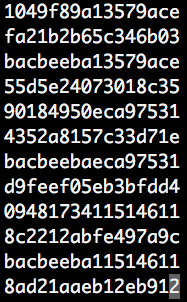
\includegraphics[height=9.06cm,width=5.61cm]{diff_src.png}
\caption{测试用明密文对}
\label{img_diff_src}
\end{figure}
\begin{figure}[htbp]
\centering
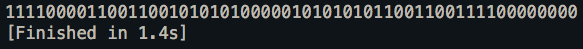
\includegraphics[height=0.98cm,width=11.66cm]{diff_key.png}
\caption{输出的56位密钥}
\label{img_diff_key}
\end{figure}

\newpage{}
\section{三重DES加解密}% finish
\subsection{简介}
三重DES提高了DES安全性,增加穷举攻击的范围。它使用两个密钥$key_1, key_2$。加密过程为,先用$key_1$加密,再用$key_2$解密,再用$key_1$加密。三重DES完全兼容DES算法(只要让两个密钥相等)。
\subsection{算法实现}
\begin{breakablealgorithm}  
    \caption{三重DES加解密}  
    \begin{algorithmic}[1] %每行显示行号  
        \Require 明文$src\_message$(加密),密钥$src\_key1, src\_key2$,密文$src\_cipher$(解密)  
        \Ensure 密文$cipher$(加密),明文$message$(解密)
        \Function {3DES\_Encrypt}{$src\_message, src\_key1, src\_key2$}
            \State $cipher1 \gets$\Call{DES\_encrypt}{$src\_message, src\_key1$}
            \State $cipher2 \gets$\Call{DES\_decrypt}{$cipher1, src\_key2$}
            \State $cipher3 \gets$\Call{DES\_encrypt}{$cipher2, src\_key1$}
            \State \Return $cipher3$
        \EndFunction

        \Function{3DES\_Decrypt}{$src\_cipher, src\_key1, src\_key2$}
            \State $message1 \gets$\Call{DES\_decrypt}{$src\_cipher, src\_key1$}
            \State $message2 \gets$\Call{DES\_encrypt}{$message1, src\_key2$}
            \State $message3 \gets$\Call{DES\_decrypt}{$message2, src\_key1$}
            \State \Return $message3$
        \EndFunction
    \end{algorithmic}  
\end{breakablealgorithm} 

\subsection{测试样例}
\begin{figure}[htbp]
\centering
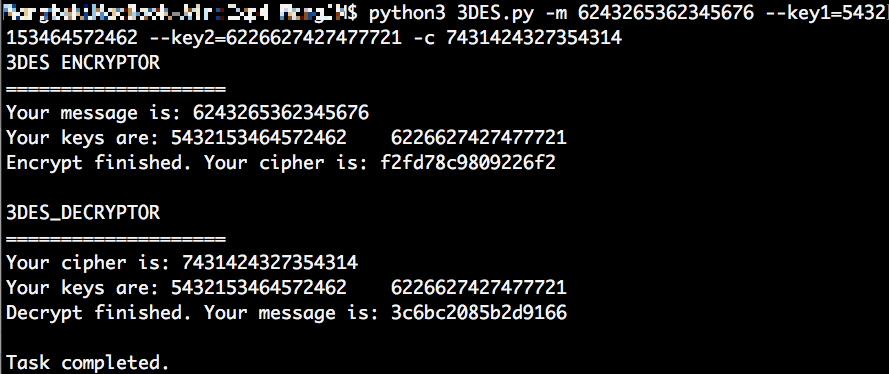
\includegraphics[height=4.48cm,width=10.67cm]{3des.png}
\caption{三重DES}
\label{img_3des}
\end{figure}

\section{二重S-DES的中间相遇攻击}
\subsection{简介}
二重DES存在中间相遇攻击的攻击方式。为了简化,采用S-DES作为示例。已知多个明密文对下,攻击流程如下:

首先,取一个明密文对,将其明文加密一次,密钥遍历所有$2^10$种可能,将所有加密结果存储起来。其次,取该明密文对的密文,将其解密一次,密钥遍历所有$2^10$种可能。如果加密结果与解密结果有重合的地方(谓之“中间相遇”),则得到相遇点的两个密钥就是可能的密钥。用其他已知的明密文对进行验证,就可以得到是否为真正密钥,从而实现攻击。

S-DES密钥很弱,事实上即使是用所有可能的明文作为检验,依然可能得到不止一组密钥,然而作为攻击者,得到两三组密钥,任务可以算是完成了。
\subsection{算法实现}
因为S-DES是DES的简化版本,简化的地方仅仅在于明文和密钥长度减少,轮数减少,因此不再在这里重写S-DES加解密伪代码。
\begin{breakablealgorithm}  
    \caption{S-DES的中间相遇攻击}  
    \begin{algorithmic}[1] %每行显示行号  
        \Require 三组明密文组(每组两对)$couple_1, couple_2, couple_3$  
        \Ensure 可能密钥对$final\_key$
        \Function {S\_DES\_MITM}{$couple_1, couple_2, couple_3$}
            \For {each $key\_1 \in [0, 1024)$}
                \State $input\_dict[$\Call{S-DES\_encrypt}{$couple1.message, key\_1$}$].append(key\_1)$
            \EndFor
        
            \For {each $key\_2 \in [0, 1024)$}
                \If {\Call{S-DES\_decrypt}{$couple_1.cipher$} $\in input\_dict.keys()$}
                    \State $maybe\_key1 = input\_dict[$\Call{S-DES\_decrypt}{$couple_1.cipher$}$]$
                    \State $maybe\_key2 = key\_2$
                    \For {each $k \in maybe\_key1$}
                        \State 用另外的明密文对检验这两个密钥
                        \If {检验正确}
                            \State $final\_key.append((k, maybe\_key2))$
                        \EndIf
                    \EndFor
                \EndIf
            \EndFor
        \State \Return $final\_key$

    \EndFunction 
    \end{algorithmic}  
\end{breakablealgorithm}
\newpage{}
\subsection{测试样例}
\begin{figure}[htbp]
\centering
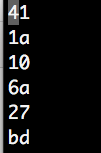
\includegraphics[height=9.18cm,width=6.06cm]{mitm_src.png}
\caption{测试用明密文对}
\label{img_mitm_src}
\end{figure}

\begin{figure}[htbp]
\centering
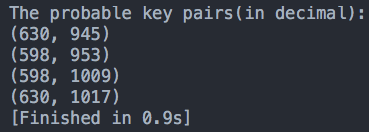
\includegraphics[height=3.96cm,width=11.07cm]{mitm_key.png}
\caption{可能的密钥对}
\label{img_mitm_key}
\end{figure}


\section{感想}
诚然,仅凭上课就完全理解DES以及各种攻击对于我而言是不现实的,事实证明通过写代码,我轻松地记住了很多关于DES的细节和攻击原理。足见代码是用来加深理解的而不是为了“实现”。因此那些不能加深理解的代码就没什么用了。

因为这次作业设计对明密文对的一类操作,所以我尝试使用了面向对象的编程方式,又尝试了命令行参数或者文件读入的IO方法。事实证明这些方式能节省很多时间。这门课让我加强了编程能力,算是一个副产品吧。

总而言之,本次实验相比前几次实验,更让我觉得有趣。
\end{document}